\documentclass[10pt]{article}

\usepackage{tikz}
\usepackage{amsmath,amsfonts,amssymb}
\usepackage{graphicx}
\usepackage{hyperref}
\usepackage{listings}
\usepackage{tikz}
\usepackage{ulem}
\usetikzlibrary{positioning,shapes,fit}
\usepackage{geometry}
\usepackage[justification=centering]{caption}
\usetikzlibrary{positioning,shapes}
\usepackage{fullpage}
\usepackage{float}

\author{Aur\`ele Barri\`ere}
\title{LRC DM 1}
\date{February 3, 2017}

\def\exercise#1{\ \vspace{1cm}\\\Large\textbf{Exercise #1}\normalsize\\}
\def\question#1{\ \vspace{1cm}\\\textbf{Question #1:}\quad}
\def\tilde{\raise.17ex\hbox{$\scriptstyle\sim$}}
\def\M{\mathcal{M}}
\def\tphi{^{\tilde\varphi}}

\def\tableau{
  \begin{figure}[H]%
    \centering
    \begin{tikzpicture}[%
        ->,
        shorten >=2pt,
        %>=stealth,
        node distance=0.4cm,
        noname/.style={%
          ellipse,
          minimum width=5em,
          minimum height=3em,
          draw
          ,thick,scale=0.4, every node/.style={transform shape}
        }
      ]
      \node[] (1) {$l\quad \neg((\Box p \wedge \Diamond q) \rightarrow \Diamond(p \wedge q))$};
      \node[] (2) [below=of 1] {\begin{tabular}{c}$l\quad \Box p\wedge\Diamond q$\\$l\quad\neg\Diamond(p\wedge q)$\end{tabular}};
      \node[] (3) [below=of 2] {$l\quad\Box(\neg p \vee \neg q)$};
      \node[] (4) [below=of 3] {\begin{tabular}{c}$l\quad\Box p$\\$l\quad\Diamond q$\end{tabular}};
      \node[] (5) [below=of 4] {\begin{tabular}{c}$R\ l\ l'$\\$l'\quad q$\end{tabular}};
      \node[] (6) [below=of 5] {$l'\quad p$};
      \node[] (7) [below=of 6] {$l'\quad \neg p \vee \neg q$};
      \node[] (8) [below left=of 7] {\begin{tabular}{c}$l'\quad\neg p$\\Contradictory\end{tabular}};
      \node[] (9) [below right=of 7] {\begin{tabular}{c}$l'\quad\neg q$\\Contradictory\end{tabular}};

      \path (1) edge [] node {} (2)
      (2) edge [] node {} (3)
      (3) edge [] node {} (4)
      (4) edge [] node {} (5)
      (5) edge [] node {} (6)
      (6) edge [] node {} (7)
      (7) edge [] node {} (8)
      (7) edge [] node {} (9);
      
  \end{tikzpicture}%
  \end{figure}
}



\def\tabdeux{
  \begin{figure}[H]%
    \scriptsize
    \centering
    \begin{tikzpicture}[%
        ->,
        shorten >=2pt,
        %>=stealth,
        node distance=0.4cm,
        noname/.style={%
          ellipse,
          minimum width=5em,
          minimum height=3em,
          draw
          ,thick,scale=0.4, every node/.style={transform shape}
        }
      ]
      \node[] (1) {$l\quad \neg(\Diamond(p\vee q) \leftrightarrow(\Diamond p\vee \Diamond q))$};
      \node[] (2) [below=of 1] {$l\quad(\neg(\Diamond (p\vee q) \rightarrow \Diamond p\vee \Diamond q) \vee\neg(\Diamond p\vee\Diamond q\rightarrow\Diamond (p\vee q)))$};
      \node[] (3) [below left=of 2] {$l\quad(\neg(\Diamond (p\vee q) \rightarrow \Diamond p\vee \Diamond q))$};
      \node[] (4) [below=of 3] {\begin{tabular}{c}$l\quad\Diamond(p\vee q)$\\$l\quad\neg(\Diamond p\vee\Diamond q)$\end{tabular}};
      \node[] (5) [below=of 4] {$l\quad \Box\neg p \wedge \Box\neg q$};
      \node[] (6) [below=of 5] {\begin{tabular}{c}$R\ l\ l'$\\$l'\quad p\vee q$\end{tabular}};
      \node[] (7) [below=of 6] {\begin{tabular}{c}$l'\quad \neg p$\\$l'\quad\neg q$\end{tabular}};
      \node[] (8) [below left=of 7] {\begin{tabular}{c}$l'\quad p$\\Contradictory\end{tabular}}; 
      \node[] (9) [below right=of 7] {\begin{tabular}{c}$l'\quad q$\\Contradictory\end{tabular}};
      \node[] (10) [below right=of 2] {$l\quad(\neg(\Diamond p\vee \Diamond q \rightarrow \Diamond (p\vee q)))$};
      \node[] (11) [below=of 10] {\begin{tabular}{c}$l\quad\Diamond p\vee\Diamond q$\\$l\quad\neg(\Diamond(p\vee q))$\end{tabular}};
      \node[] (12) [below=of 11] {$l\quad\Box(\neg p\wedge\neg q)$};
      \node[] (13) [below left=of 12] {$l\quad\Diamond p$};
      \node[] (14) [below=of 13] {\begin{tabular}{c}$R\ l\ l'$\\$l'\quad p$\end{tabular}};
      \node[] (15) [below=of 14] {$l'\quad\neg p\wedge\neg q$};
      \node[] (16) [below=of 15] {\begin{tabular}{c}$l'\quad\neg p$\\Contradictory\end{tabular}};
      \node[] (17) [below right=of 12] {$l\quad\Diamond q$};
      \node[] (18) [below=of 17] {\begin{tabular}{c}$R\ l\ l'$\\$l'\quad q$\end{tabular}};
      \node[] (19) [below=of 18] {$l'\quad\neg p\wedge\neg q$};
      \node[] (20) [below=of 19] {\begin{tabular}{c}$l'\quad\neg q$\\Contradictory\end{tabular}};

      \path (1) edge [] node {} (2)
      (2) edge [] node {} (3)
      (3) edge [] node {} (4)
      (4) edge [] node {} (5)
      (5) edge [] node {} (6)
      (6) edge [] node {} (7)
      (7) edge [] node {} (8)
      (7) edge [] node {} (9)
      (2) edge [] node {} (10)
      (10) edge [] node {} (11)
      (11) edge [] node {} (12)
      (12) edge [] node {} (13)
      (13) edge [] node {} (14)
      (14) edge [] node {} (15)
      (15) edge [] node {} (16)
      (12) edge [] node {} (17)
      (17) edge [] node {} (18)
      (18) edge [] node {} (19)
      (19) edge [] node {} (20);


      
    \end{tikzpicture}
  \end{figure}
}

\def\hilbert{
\begin{tabular}{l l l}
1 & $\Box(p\rightarrow\neg q)\rightarrow(\Box p\rightarrow\Box\neg q)$ & Modal distributivity\\
2 & $\neg\neg\Box(p\rightarrow\neg q)\rightarrow\neg\neg(\Box p\rightarrow\Box\neg q)$ & Rewriting 1\\
3 & $(\neg\neg\Box(p\rightarrow\neg q)\rightarrow\neg\neg(\Box p\rightarrow\Box\neg q))\rightarrow(\neg(\Box p\rightarrow\Box\neg q)\rightarrow(\neg\Box(p\rightarrow\neg q)))$ & Axiom 3\\
4 & $\neg(\Box p\rightarrow\Box\neg q)\rightarrow(\neg\Box(p\rightarrow\neg q))$ & Modus Ponens on 2,3\\
5 & $(\Box p\wedge\Diamond q)\rightarrow\Diamond(p\wedge q)$ & Rewriting the $\neg$ in 4 
\end{tabular}
}

\def\hilbertdeux{
We will prove the two implications separately.

\paragraph{First lemma:} $\Box(\varphi\wedge\psi)\rightarrow(\Box\varphi\wedge\Box\psi)$

\begin{tabular}{l l l}
1 & $\varphi\wedge\psi\rightarrow\varphi$ & (PL3)\\
2 & $\Box(\varphi\wedge\psi\rightarrow\varphi)$ & Necessitation with 1\\
3 & $\Box((\varphi\wedge\psi)\rightarrow\varphi)\rightarrow(\Box(\varphi\wedge\psi)\rightarrow\Box\varphi)$ & Modal distributivity\\
4 & $\Box(\varphi\wedge\psi)\rightarrow\Box\varphi$ & Modus Ponens on 2,3\\
5 & $\varphi\wedge\psi\rightarrow\psi$ & (PL3)\\
6 & $\Box(\varphi\wedge\psi\rightarrow\psi)$ & Necessitation with 5\\
7 & $\Box((\varphi\wedge\psi)\rightarrow\psi)\rightarrow(\Box(\varphi\wedge\psi)\rightarrow\Box\psi)$ & Modal distributivity\\
8 & $\Box(\varphi\wedge\psi)\rightarrow\Box\psi$ & Modus Ponens on 6,7\\
9 & $((\Box(\varphi\wedge\psi)\rightarrow\Box\varphi)\wedge(\Box(\varphi\wedge\psi)\rightarrow\Box\psi))\rightarrow(\Box(\varphi\wedge\psi)\rightarrow(\Box\varphi\wedge\Box\psi))$ & (PL1)\\
10 & $\Box(\varphi\wedge\psi)\rightarrow(\Box\varphi\wedge\Box\psi)$ & Modus Ponens on 4,8,9
\end{tabular}

\paragraph{First implication:} $\Diamond p\vee\Diamond q\rightarrow\Diamond(p\vee q)$

\begin{tabular}{l l l}
1 & $\Box(\neg p\wedge\neg q)\rightarrow(\Box\neg p\wedge\Box\neg q)$ & By the previous lemma\\
2 & $\neg\neg\Box(\neg p\wedge\neg q)\rightarrow\neg\neg(\Box\neg p\wedge\Box\neg q)$ & Rewriting 1\\
3 & $(\neg\neg\Box(\neg p\wedge\neg q)\rightarrow\neg\neg(\Box\neg p\wedge\Box\neg q)) \rightarrow (\neg(\Box\neg p\wedge\Box\neg q)\rightarrow\neg\Box(\neg p\wedge\neg q))$ & Axiom 3\\
4 & $\neg(\Box\neg p\wedge\Box\neg q)\rightarrow\neg\Box(\neg p\wedge\neg q)$ & Modus Ponens on 2,3\\
5 & $\Diamond p\vee\Diamond q\rightarrow\Diamond(p\vee q)$ & Rewriting $\neg$ in 4
\end{tabular}

\paragraph{Second lemma:} $\Box\varphi\wedge\Box\psi\rightarrow\Box(\varphi\wedge\psi)$

\begin{tabular}{l l l}
1 & $\varphi\rightarrow(\psi\rightarrow(\varphi\wedge\psi))$ & (PL2)\\
2 & $\Box(\varphi\rightarrow(\psi\rightarrow(\varphi\wedge\psi)))$ & Necessitation\\
3 & $\Box(\varphi\rightarrow(\psi\rightarrow(\varphi\wedge\psi)))\rightarrow(\Box\varphi\rightarrow\Box(\psi\rightarrow(\varphi\wedge\psi)))$ & Modal distributivity\\
4 & $\Box\varphi\rightarrow\Box(\psi\rightarrow(\varphi\wedge\psi))$ & Modus Ponens on 2,3\\
5 & $(\Box\varphi\rightarrow\Box(\psi\rightarrow(\varphi\wedge\psi)))\rightarrow(\Box\varphi\rightarrow(\Box\psi\rightarrow(\Box(\varphi\wedge\psi))))$ & Modal distributivity and Modus Ponens\\
6 & $\Box\varphi\rightarrow(\Box\psi\rightarrow(\Box(\varphi\wedge\psi)))$ & Modus Ponens on 4,5\\
7 & $\Box\varphi\wedge\Box\psi\rightarrow\Box(\varphi\wedge\psi)$ & Modus Ponens on 6 and (PL5)
\end{tabular}

\paragraph{Second implication:} $\Diamond (p\vee q)\rightarrow\Diamond p\vee\Diamond q$

\begin{tabular}{l l l}
1 & $(\Box\neg p\wedge\Box\neg q) \rightarrow\Box(\neg p\wedge\neg q)$ & By the previous lemma\\
2 & $\neg\neg(\Box\neg p\wedge\Box\neg q) \rightarrow\neg\neg\Box(\neg p\wedge\neg q)$ & Rewriting 1\\
3 & $(\neg\neg(\Box\neg p\wedge\Box\neg q) \rightarrow\neg\neg\Box(\neg p\wedge\neg q)) \rightarrow (\neg\Box(\neg p\wedge\neg q)\rightarrow\neg(\Box\neg p\wedge\Box\neg q))$ & Axiom 3\\
4 & $\neg\Box(\neg p\wedge\neg q)\rightarrow\neg(\Box\neg p\wedge\Box\neg q)$ & Modus Ponens on 2,3\\
5 & $\Diamond (p\vee q)\rightarrow\Diamond p\vee\Diamond q$ & Rewriting $\neg$ in 4
\end{tabular}

}

\def\counterexample{
  \begin{figure}
    \centering
    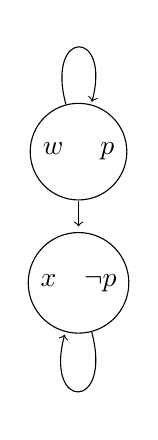
\begin{tikzpicture}[%
        ->,
        shorten >=2pt,
        %>=stealth,
        node distance=0.4cm,
        noname/.style={%
          ellipse,
          minimum width=5em,
          minimum height=3em,
          draw
          ,thick,scale=0.4, every node/.style={transform shape}
        }
      ]
      \node[circle,draw] (1) {$w\quad\ p$};
      \node[circle,draw] (2) [below=of 1] {$x\quad\neg p$};
      \path (1) edge [] node {} (2)
      (2) edge [loop below] node {} (2)
      (1) edge [loop above] node {} (1);
  \end{tikzpicture}%
    \caption{Exercise 2 question 2: An example where the formula $p\rightarrow\Box\Diamond p$ isn't true}
    \label{2.2}
  \end{figure}
}

\def\nottransitive{
  \begin{figure}%
    \centering
    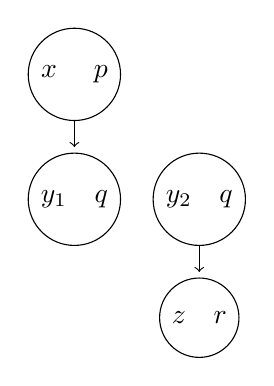
\begin{tikzpicture}[%
        ->,
        shorten >=2pt,
        %>=stealth,
        node distance=0.4cm,
        noname/.style={%
          ellipse,
          minimum width=5em,
          minimum height=3em,
          draw
          ,thick,scale=0.4, every node/.style={transform shape}
        }
      ]
      \node[circle,draw] (1) {$x\quad\ p$};
      \node[circle,draw] (2) [below=of 1] {$y_1\quad q$};
      \node[circle,draw] (3) [right=of 2] {$y_2\quad q$};
      \node[circle,draw] (4) [below=of 3] {$z\quad r$};
      \path (1) edge [] node {} (2)
      (3) edge [] node {} (4);
  \end{tikzpicture}%
 \hspace{3cm}
    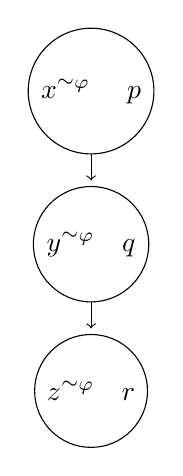
\begin{tikzpicture}[%
        ->,
        shorten >=2pt,
        %>=stealth,
        node distance=0.4cm,
        noname/.style={%
          ellipse,
          minimum width=5em,
          minimum height=3em,
          draw
          ,thick,scale=0.4, every node/.style={transform shape}
        }
      ]
      \node[circle,draw] (1) {$x\tphi\quad\ p$};
      \node[circle,draw] (2) [below=of 1] {$y\tphi\quad q$};
      \node[circle,draw] (3) [below=of 2] {$z\tphi\quad r$};
      \path (1) edge [] node {} (2)
      (2) edge [] node {} (3);
  \end{tikzpicture}%
    \caption{Exercise 4: Not every filtration of a transitive model is transitive}
    \label{4}
  \end{figure}
}





\begin{document}
\maketitle

\exercise{1}
\question{1} 
We show that the two Kripke models are bisimilar by giving a bisimulation relation between the two.
Let $R_{a1}, R_{b1}$ be the accessibility relations of the first Kripke model, and $R_{a2}, R_{b2}$ the accessibility relations of the second one.

Consider $Z$ the following binary relation :
$$\left\{
\begin{array}{l}
\forall n\in\mathbb{N},\quad w\ Z\ w^n \\
\forall n\in\mathbb{N},\quad v\ Z\ v^n
\end{array} 
\right.$$

Let's show that the relation $Z$ is a bisimulation.
\paragraph{Atom} Every world in each Kripke model make true the same propositional letter  : $p$, and only this one. 

\paragraph{Forth} Let $n\in\mathbb{N}$. We have $w\ Z\ w^n$. The only successor of $w$ in the first Kripke model is $v$ : $w\ R_{a1}\ v$. We also have $w^n\ R_{a2}\ v^n$. And by definition of $Z$, $v\ Z\ v^n$.

Let $n\in\mathbb{N}$. We have $v\ Z\ v^n$. The only successor of $v$ in the first Kripke model is $w$ : $v\ R_{b1}\ w$. We also have $v^n\ R_{b2}\ w^{n+1}$. And by definition of $Z$, $w\ Z\ v^{n+1}$.

Thus, the \textit{Forth} rule is true for $Z$, as every pair in relation with $Z$ is either $w\ Z\ w^n$ or $v\ Z\ v^n$ by definition.

\paragraph{Back} Let $n\in\mathbb{N}$. We have $w\ Z\ w^n$. The only successor of $w^n$ in the first Kripke model is $v^n$. We also have $w\ R_{a1}\ v$ and $v\ Z\ v^n$. 

 Let $n\in\mathbb{N}$. We have $v\ Z\ v^n$. The only successor of $v^n$ in the first Kripke model is $w^{n+1}$. We also have $v\ R_{b1}\ w$ and $w\ Z\ w^{n+1}$. 

\paragraph{Conclusion} $Z$ is a non-empty bisimulation between the two Kripke models. The two Kripke models are thus bisimilar.


\question{2} The smallest Kripke model bisimilar to $\M$ must have at least one world, for the bisimulation to be non-empty.

The Kripke model with only one world in which the propositional letter $t$ is true is bisimilar to $\M$. Let $w$ be this world.

We then define $Z$ the bisimulation such that $9\ Z\ w$. $Z$ is a bisimulation : in both $9$ and $w$, only $t$ is true, and both $9$ and $w$ have no successors. And this Kripke model is the smallest possible as it only has one world.

The Kripke contraction is thus $(\{w\},\emptyset,V)$ such that $V(w,t)=\mathit{true}$.


\question{3}

\paragraph{Union of two bisimulations} We will first prove that the union of two bisimulations is a bisimulation.
Let $Z_1$ and $Z_2$ be two bisimulations between $\M$ and $\M'$. Let $Z=Z_1\cup Z_2$.

\textit{Atom} is true for $Z$. Indeed, whenever $w\ Z\ v$, either $w\ Z_1\ v$ or $w\ Z_2\ v$. In each case, we have that $w$ and $v$ make true the same propositional letters because $Z_1$ and $Z_2$ are bisimulations.

\textit{Forth} is true for $Z$. Consider the case where $w\ Z_1\ v$ (the case with $Z_2$ is the same). In that case, forall $w'$ such that $w\ R\ w'$, there exists some $v'$ such that $v\ R\ v'$ and $w'\ Z_1\ v'$. Then by definition of $Z$, we also have $w'\ Z\ v'$.
\textit{Back} is also true for $Z$ : the proof is symmetrical.

Thus, $Z$ is a bisimulation between $\M$ and $\M'$.

\paragraph{Finite number of bisimulations} Then, we show that between two finite Kripke frames, there exists only a finite number of bisimulation. Indeed, a bisimulation is included in the set $\mathcal{W}^\M\times\mathcal{W}^{\M'}$, which is finite.

\paragraph{Union of bisimulations} We can now deduce that any non-empty union of bisimulations is a bissimulation recursively on the number of bisimulations in the collection. Since this number is finite, and because the union of two bisimulations is one too, then we have that the union of the whole collection is a bisimulation as well.

\paragraph{Maximal bisimulation} Let $Z_m = \underset{X \mathit{bisimulation}}{\bigcup} X$. The union is finite because there only is a finite number of bisimulations. There is always at least one bisimulation between two Kripke models : $\emptyset$. We can thus apply the previous result and deduce that $Z_m$ is a bisimulation. Moreover, for each bisimulation $X$, by definition of $Z_m$, we have $X\subseteq Z_m$. Thus, $Z_m$ is a maximal bisimulation.



\exercise{2}
\question{1}
We present a proof using the tableau method and another one in the Hilbert system for each formula.

\question{1.1}

\tableau

\hilbert

\question{1.2}

\tabdeux

\hilbertdeux



\question{2}
\paragraph{Unprovability in \textbf{S4}} To show that $p\rightarrow\Box\Diamond p$ cannot be proved in \textbf{S4}, we give a Kripke model that verify the hypothesis of \textbf{S4} (reflexivity and transitivity) in which the formula is not true. We then conclude with the soundness of the deductive system that, if the formula was provable, then it would hold in our exemple.

We define $\M=(\{w,x\},R,V)$ where $w\ R\ w$, $x\ R\ x$ and $w\ R\ x$. $V$ is such that $V(x,p)=\mathit{true}$ and $V(w,p)=\mathit{false}$. $\M$ is transitive and reflexive. We have that $\M,w\not\models p\rightarrow\Box\Diamond p$, as $\M,w\models p$ but $\M,x\not\models\Diamond p$. We show $\M$ in \textsc{Figure}\ \ref{2.2}.

As \textbf{S4} is sound for models with a reflexive and transitive relation, the formula is unprovable.

\counterexample

\paragraph{Proof in \textbf{S5}} 

\begin{tabular}{l l l}
1 & $p\rightarrow\Diamond p$ & Reflexivity Axiom\\
2 & $\Diamond p\rightarrow\Box\Diamond p$ & S5 Axiom\\
3 & $p\rightarrow\Box\Diamond p$ & $(i)$ on 1,2\\
\end{tabular}

We still need to prove $(i)$ : $\frac{P\rightarrow Q\quad Q\rightarrow R}{P\rightarrow R}$.

TODO : prove $(i)$ (cut cannot be proved easily...)

\question{3}
Let $\M$ be a transitive and reflexive Kripke model.
Let $w$ be a world in $\M$, such that $\M,w\models\Box\Diamond\Box\Diamond\varphi$.

Then, forall $w_1$ such that $w\ R\ w$, there exists some $w_2$ such that $w_1\ R\ w_2$ and forall $w_3$ such that $w_2\ R\ w_3$, there exists $w_4$ such that $w_3\ R\ w_4$ and $w_4\models\varphi$.

Let $v_1$ be a successor of $w$ in $\M$. By assumption, there exists some $w_2$, such that $v1\ R\ w_2$, and $w_2\models\Box\Diamond\varphi$. 
Let $w_3$ be a successor of $w_2$. $w_3$ exists because $\M$ is reflexive.
By assumption, there exists some $w_4$ such that $w_4\models\varphi$ and $w_3\ R\ w_4$.

By transitivity of $\M$, we also have $v_1\ R\ w_4$, because $v_1\ R\ w_2$ and $w_2\ R\ w_3$ and $w_3\ R\ w_4$.

Thus, for each successor $v_1$ of $w$, we can find a successor of $v_1$ that satisfies $\varphi$.

Thus, $\M,w\models\Box\Diamond\varphi$.

Finally, we have that in a relfexive and transitive Kripke model,
$$\Box\Diamond\Box\Diamond\varphi\rightarrow\Box\Diamond\varphi$$.

\exercise{3}
Let $p$ be a propositional letter.
Assume that there exists some $\varphi$, such that for all pointed Kripke model $(\M,w)$, we have $\M,w\models\varphi\leftrightarrow\M,w\models D_p$.

$\varphi$ cannot be true in every pointed Kripke model. Indeed, it would mean that $D_p$ is also true in every pointed Kripke model which is impossible : consider the Kripke model with only one world where $p$ is false.

Thus, there exists at least one pointed Kripke model $\M,w$ such that $\M,w\models\neg\varphi$ and thus $\M,w\models\neg D_p$.
Let $\M' = (W^\M\cup\{w_p\}, R^\M, V^\M[V(w_p,p)=\mathit{true}])$, in which $w_p$ is a new world added to $\M$ where $p$ is true.

We have that $\M$ and $\M'$ are bisimilar : the relation that links any world of $\M$ with its copy in $\M'$ is a bisimulation, because $\M'$ is just a copy of $\M$ with a new disconnected world. Thus every world of $\M$ and its copy in $\M'$ make true the same formulas.

We have $\M',w\models D_p$ by definition of $D_p$, because $\M',w_p\models p$.
But $\M',w\models\neg\varphi$, because $\M,w\models\neg\varphi$, and $w\in\M$ and $w\in\M'$ make true the same modal formulas.  Which means that the difference is not defined by $\varphi$.

Thus we have shown that one cannot define a Modal Logic formula that expresses the difference operator for a propositional letter (and therefore the difference operator cannot be defined for every formula).


\exercise{4}
\question{1}
Let us define a transitive Kripke model $\M$ and a formula $\varphi$, such that $\M\tphi$ isn't transitive.

Let $\M = (W,R,V)$ such that $W=\{x,y_1,y_2,z\}$, $R = \{(x,y_1),(y_2,z)\}$ and $V(x)=p$, $V(y_1)=V(y_2)=q$ and $V(z)=r$. Let $\varphi=p\wedge q\wedge r$.

In  $\M\tphi$, there are 3 worlds : $x\tphi=\{x\}$, $y_1\tphi=\{y_1,y_2\}$ and $z\tphi=\{z\}$.

We also have $x\tphi\ R\tphi\ y_1\tphi$ and $y_1\tphi\ R\tphi\ z\tphi$, but we don't have $x\tphi\ R\tphi\ z\tphi$, which means that $\M\tphi$ isn't transitive. We show $\M$ and $\M\tphi$ \textsc{Figure}\ \ref{4}.

We thus deduce that not every filtration of a transitive Kripke model is transitive.

\nottransitive


\question{2}
Let $\M$ be a transitive Kripke model. Let's show that, using the new relation, $\M\tphi$ is transitive.

Let $x\tphi, y\tphi$ and $z\tphi$ $\in W\tphi$ such that $x\tphi\ R\tphi\ y\tphi$ and $y\tphi\ R\tphi\ z\tphi$. If no such worlds exists, then $\M\tphi$ is trivially transitive. Let us show that $x\tphi\ R\tphi\ z\tphi$ which would mean that $\M\tphi$ is transitive.

As we have $x\tphi\ R\tphi\ y\tphi$, then forall $\psi$ such that $\Diamond\psi\in\mathit{Sub}(\varphi)$, if $\M,y\models\psi\vee\Diamond\psi$ then $\M,x\models\Diamond\psi$ by definition of the new relation of $\M\tphi$. (1)

We also have $y\tphi\ R\tphi\ z\tphi$, then forall $\psi$ such that $\Diamond\psi\in\mathit{Sub}(\varphi)$, if $\M,z\models\psi\vee\Diamond\psi$ then $\M,y\models\Diamond\psi$. (2)

To show that $x\tphi\ R\tphi\ z\tphi$, let us take $\psi$ such that $\Diamond\psi\in\mathit{Sub}(\varphi)$ and $\M,z\models\psi\vee\Diamond\psi$. If no such $\psi$ exists, then we trivially have $x\tphi\ R\tphi\ z\tphi$. Let us show $\M,x\models\Diamond\psi$.

Using (2), we have that $\M,y\models\Diamond\psi$. Then we have $\M,y\models\psi\vee\Diamond\psi$ by defnitiion of $\models$. Then using (1), we deduce that $\M,x\models\Diamond\psi$. We thus have $x\tphi\ R\tphi\ z\tphi$.

Then, we have shown that $\M\tphi$ is transitive. We deduce that any filtration of a transitive model is transitive using this relation. As we did not use the transitivity of $\M$ in our proof, we can also deduce that the filtration with the new relation of any Kripke model is transitive.

\exercise{5}
\question{1}
\paragraph{The first-order formula implies the modal formula:}
Let $\M$ be a Kripke model which satisfies the first-order formula. Let $x$ be a world of $\M$. Let's show that $\M,x\models\Diamond(\Diamond p\wedge\Box q)\rightarrow\Box(\Diamond p\vee\Box q)$.

If $\M,x\not\models\Diamond(\Diamond p\wedge\Box q)$, then the implication is verified. If $\M,x\models\Diamond(\Diamond p\wedge\Box q)$, then there exists some $y_1$, such that $x\ R\ y_1$ and $\M,y_1\models(\Diamond p\wedge\Box q)$. Let $y_2$ be a world of $\M$ such that $x\ R\ y_2$. Let's show that $\M,y_2\models\Diamond p\vee\Box q$.

We can use the first-order formula to deduce that we have $(\forall z,y_1\ R\ z\rightarrow y_2\ R\ z)$ or $(\forall z,y_2\ R\ z\rightarrow y_1\ R\ z)$.
In the case where $\forall z,y_1\ R\ z\rightarrow y_2\ R\ z$, then every successor of $y_1$ is a successor of $y_2$. As we had $y_1\models\Diamond p\wedge\Box q$, we have that $\M,y_1\models\Diamond p$, then there exists some $z$ such that $y_1\ R\ z$ and $\M,z\models p$. With the first-order formula, we have that $y_2\ R\ z$, which means $\M,y_2\models\Diamond p$, and thus $\M,y_2\models\Diamond p\vee\Box q$.
In the case where $\forall z,y_2\ R\ z\rightarrow y_1\ R\ z$, then every successor of $y_2$ is a successor of $y_1$. Let $z$ be a successor of $y_2$. It is a successor of $y_1$ and thus $\M,z\models q$ as $\M,y_1\models\Box q$. Then $\M,y_2\models\Box q$ and thus $\M,y_2\models\Diamond p\vee\Box q$.

In both cases, we have that for any successor $y_2$ of $x$ in $\M$, $\M,y_2\models\Diamond p\vee\Box q$. Which means that $\M,x\models\Diamond(\Diamond p\wedge\Box q)\rightarrow\Box(\Diamond p\vee\Box q)$. It shows that any model that makes true the first-order formula also makes true the modal formula (E).

 
\paragraph{The modal formula implies the first-order formula}
Let $F$ be a Kripke frame in which $\forall x\in F,\forall V, (F,V),x\models\Diamond(\Diamond p\wedge\Box q)\rightarrow\Box(\Diamond p\vee\Box q)$. Let $x,y_1,y_2$ be worlds of $F$ such that $x\ R\ y_1$ and $x\ R\ y_2$. Let us show that either $\forall z, y_1\ R\ z\rightarrow y_2\ R\ z$ or $\forall z, y_2\ R\ z\rightarrow y_1\ R\ z$.

Let's assume the negation : $\exists z_1,z_2, (y_1\ R\ z_1), (y_2\ R\ z_2), \neg(y_1\ R\ z_2), \neg(y_2\ R\ z_1)$. For the valuation $V$ such that $p$ is true only in $z_1$ and false everywhere else, and $q$ is false in $z_2$ and true everywhere else, we have that $(F,V),x\models\Diamond(\Diamond p\wedge\Box q)$, because $(F,V),y_1\models(\Diamond p\wedge\Box q)$. However, $(F,V)\not\models\Box(\Diamond p\vee\Box q)$ because in $y_2$ there is no successor that satisfies $p$ (because only $z_1$ satisfies $p$ and $\neg(y_2\ R\ z_1)$) and there is one successor, $z_2$, in which $q$ is false.

Thus, we have proved that (E) corresponds to the first-order formula, which means that the class of frames that satisfies (E) is exactly the class of frames that satisfies the first-order formula.

\question{2}

\paragraph{$Q$ implies $R^{-1}\subseteq R^*$:}
We want to show that for every Kripke frame $F$, if $F$ validates $T,E$ and $Q$ for any valuation, then $R^{-1}\subseteq R^*$. Let us assume the opposite and show that it isn't possible.

Assume that there exists some frame $F$, such that $F$ validates $T,E$ and $Q$ for any valuation, but there also exists $s$ an $t$ in $F$ such that $s\ R\ t$ but there exists no finite path from $t$ to $s$.
Start by noticing that necessarily, $s\neq t$ or there would exist such a finite path from $t$ to $s$.

Let us consider the valuation $V$ where the propositionnal letter $p$ is true in $t$, true in the succssors of $t$ ($R(t)$), true in their successors\dots true in any world that can be reached from $t$ and only in them ($R^*(t)$). Obviously, $s$ isn't one of these worlds, or else it would mean that there exists a path from $t$ to $s$.


In this Kripke world, we have that $(F,V),s\models\Diamond p$, because $t$ is a successor of $s$ in which $p$ is true. 

We also have $(F,V),s\models\Box(p\rightarrow\Box p)$, because in each successor of $s$, $p\rightarrow\Box p$ is true. Let us show that last point. Let $u$ be a successor of $s$.

\begin{itemize}
\item If $u=s$, then the implication is true because $(F,V),s\not\models p$.
\item If $u\in R^*(t)$, then the implication is true because $p$ is true in $u$ and in each of its successors (because they also are in $R^*(t)$).
\item If $u\not\in R^*(t)$, then the implication is true because $(F,V),u\not\models p$.
\end{itemize}

We thus have that $(F,V),s\models (\Diamond p\wedge\Box(p\rightarrow\Box p))$, but $(F,V),s\not\models p$, which is in contradiction with the fact that $F$ satisfies $(Q)$.

We thus have that in a frame that satisfies $T,E$ and $Q$, $R^{-1}\subseteq R^*$.


\paragraph{$R^{-1}\subseteq R^*$ implies $Q$:}
Let $\M$ be a Kripke model in which $R^{-1}\subseteq R^*$, that satisfies both $T$ and $E$. Let us show that $Q$ holds in $\M$.

Let $s\in\M$, such that $\M,s\models(\Diamond p\wedge\Box(p\rightarrow\Box p))$. Let us show that $p$ holds in $s$. As $\M,s\models\Diamond p$ there is some $u_0$, a successor of $s$ in which $p$ is true. As $R^{-1}\subseteq R^*$, there exists $u_1,u_2\dots u_m$ the shortest finite path to $s$ from $u_0$.

Let us show recursively that $\forall i\in[0,m], V(u_i,p)=\mathit{true\ } \text{ and\ } s\ R\ u_i$.

It is true for $u_0$.
If it is true for $u_n$ where $n<m$, then let us show that it is also true for $u_{n+1}$.

As $s$ and $u_n$ are both successors of $s$ by inductive hypothesis, then, using the question 1 and because $\M$ satisfies $E$, either $R(s)\subseteq R(u_n)$ or $R(u_n)\subseteq R(s)$. If $R(s)\subseteq R(u_n)$, then we have $u_n\ R\ s$ because $s\in R(s)$ (as $\M$ is reflexive because it satisfies $T$). This is absurd because we said that $u_1\dots u_m$ was the shortest path, not $u_1\dots u_n$. In the other case, we have that $R(u_n)\subseteq R(s)$, which implies that $s\ R\ u_{n+1}$. We also have that $p$ is true in $u_{n+1}$ because $\M,s\models\Box(p\rightarrow\Box p)$ and $u_n\in R(s)$. Our hypothesis is thus proved recursively.

Which means that we have $s\ R\ u_m$ (and also $u_m\ R\ s$ because $s$ concludes the finite path), and $p$ is true in $u_m$. As $\Box(p\rightarrow\Box p)$ is true in $s$, then $p\rightarrow\Box p$ is true in $u_m$ and finally, $p$ is true in $s$.

\paragraph{Conclusion}
We have shown that in the class of frames that satisfies both $T$ and $E$, a frame satisfies also $Q$ iff $R^{-1}\subseteq R^*$. It means that in the class of frames validating $T$ and $E$, $Q$ defines the sub-class of frames in which $R^{-1}\subseteq R^*$ is true.

\question{3}
Let us write $P$ the property $P\ :\ \forall x,(x\ R\ y\leftrightarrow x=y)$.

\paragraph{$P$ implies $T\wedge M\wedge E\wedge Q$:}
Let $F$ be a Kripke frame that validates $P$. Let us show that $T\wedge M\wedge E\wedge Q$ is verified too for every valuation.
\begin{itemize}
\item $T$ : Because $T$ defines the class of reflexive Kripke frames.
\item $M$ : If $p$ is true in a world, then $\Diamond\Box p$ is true, and if $p$ is false then $\Box\Diamond p$ is false. Thus, the implication is true in each world regardless of the valuation.
\item $E$ : The first-order formula given in the first question is verified because every successor of a world is the node itself.
\item $Q$ : If $p$ is true in a world, then the implication holds. When $p$ is false, $\Diamond p$ is also false, then the premise of the implication is false and thus the implication holds.
\end{itemize}

We thus have that $P$ implies $T\wedge M\wedge E\wedge Q$.

\paragraph{$T\wedge M\wedge E\wedge Q$ implies $P$:}

\paragraph{Lemma: another definition for $M$}
We show here that $M$ defines the class of Kripke frames in which for each node that has at least one successor, one of its successors does not have strictly more thatn one successor itself. We'll note this property $N$.

First, we have that $N$ implies $M$. Indeed let us take $F$ a Kripke frame in which $N$ is true.

Then, let us show that $M$ implies $N$.
TODO


\paragraph{Proving the trivial accessibility relation} Let $\M$ be a Kripke frame that validates $T,M,E$ and $Q$ for every valuation $V$. Let us show that $F$ also validates $P$.

Let $x,y\in\M$. If $x=y$, then we have $x\ R\ y$ because $F$ is reflexive as it validates $T$.
Now let us show that a world is its only successor.

Let $x\in\M$. As $F$ validates $M$, and $x$ has at least one successor (itself), we know that there is some $y\in R(x)$ such that $y$ has at most one successor. Because of the relflexivity of $F$, this successor is $y$ itself. We will show that $x=y$. Indeed, if $y$ was different from $x$, then there would be no finite path from $y$ to $x$ because $R(y)=\{y\}$. And $F$ validates $T,E$ and $Q$ which means that such a path should exist.

We then deduce that $x=y$. $x$ is then its successor that can have at most one successor : itself. It is thus impossible for $x$ to have another successor.

\paragraph{Conclusion}
Thus, we have proved that the class of frames which validates $T,M,E$ and $Q$ are exactly the Kripke frames with a trivial accessibility relation.

\end{document}
